\begin{figure}
    \centering
    \begin{subfigure}[b]{\textwidth}
        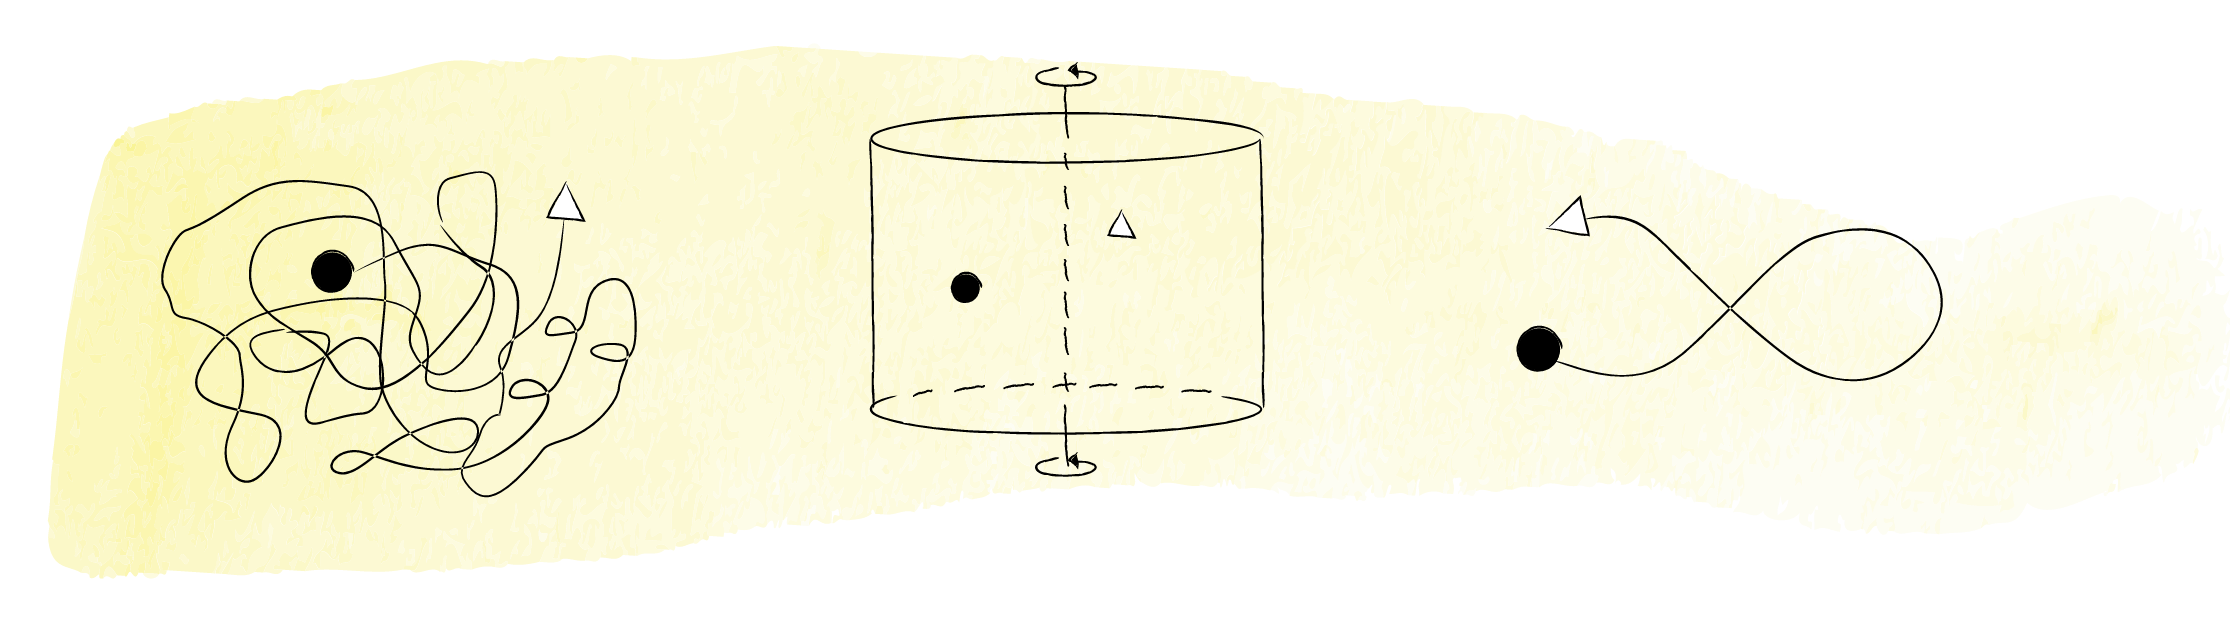
\includegraphics[width=\textwidth]{FishPoo/figures/change_of_basis_a}
        \small
        \caption{A rotating frame}
    \end{subfigure}\\
    \begin{subfigure}[b]{\textwidth}
        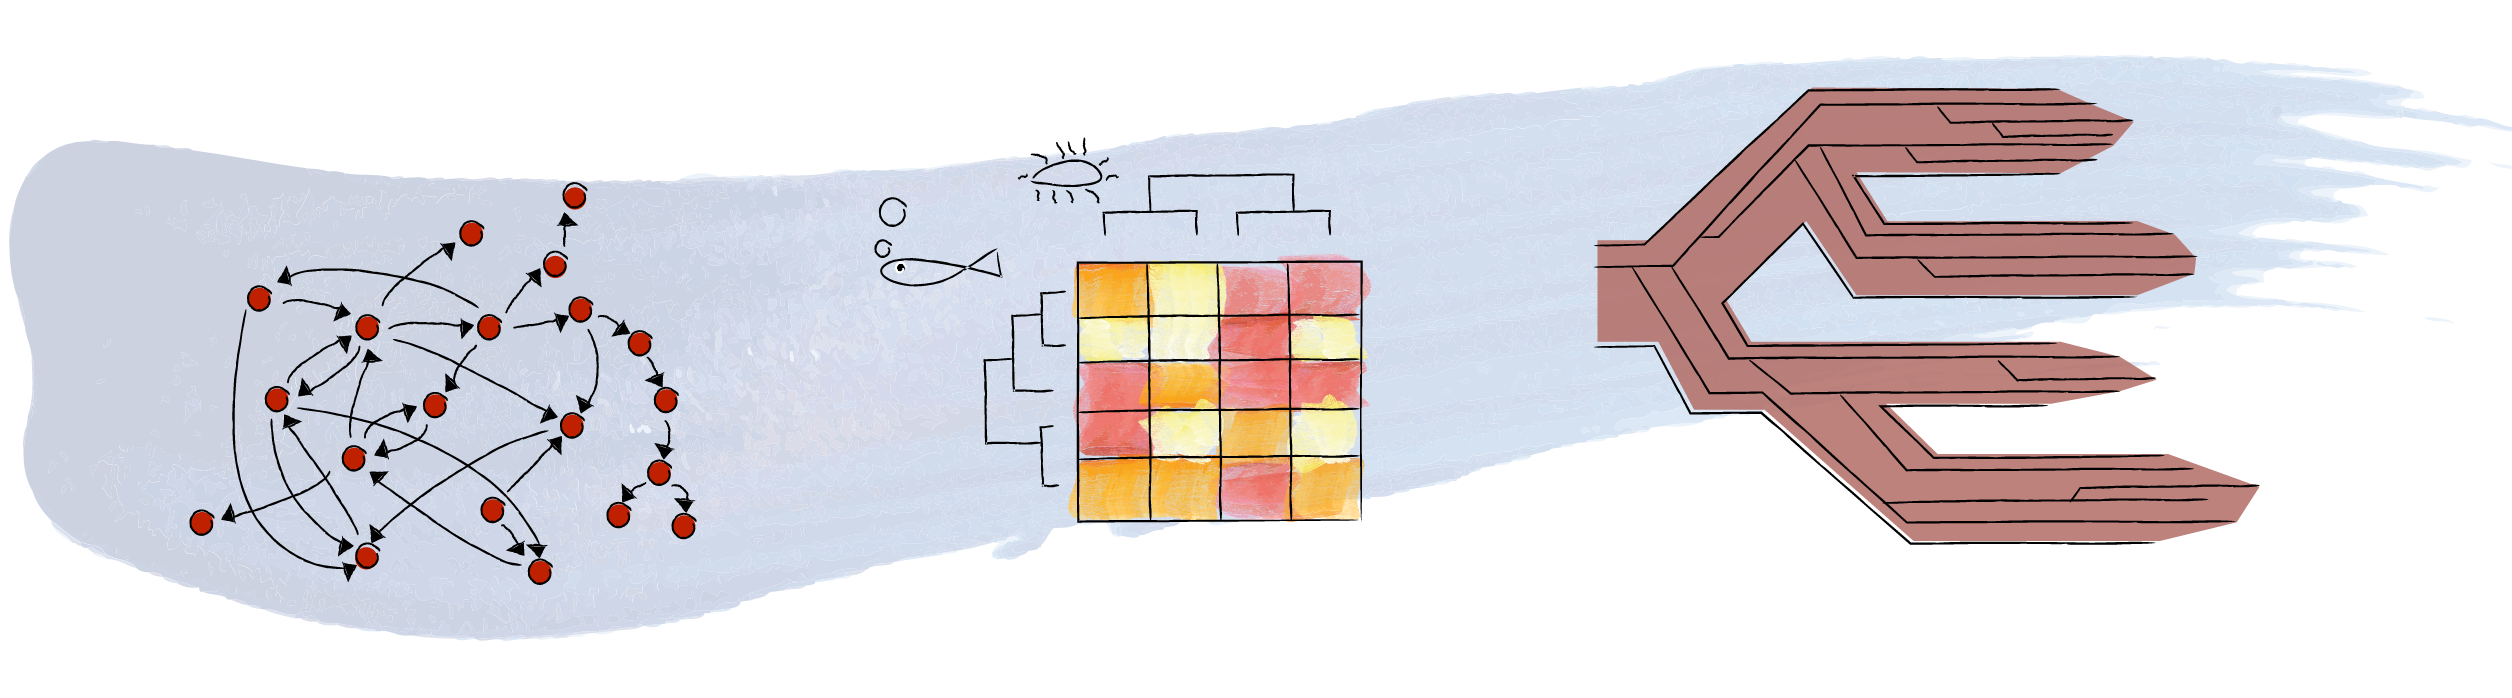
\includegraphics[width=\textwidth]{FishPoo/figures/change_of_basis_b}
        \small
        \caption{An evolving host}
    \end{subfigure}
    \caption{A change of basis can simplify a trajectory by separating the contributions of different processes. In the case of motion in a rotating frame \textbf{(a)}, re-expressing the trajectory within the rotating frame is a useful change of basis. In the case of ecological interactions among microbes \textbf{(b)}, re-expressing their phylogenies in the context of the evolution of their hosts can also be a useful change of basis. }
    \label{fig:FP_change_of_basis}
\end{figure}
